\clearpage
\section{Previous searches}
\label{sec:previous-searches}

Since Higgsinos solve puzzles and shortcomings in the SM, there have been numerous attempts to discover them at the LHC and previous colliders. These searches resulted in exclusion limits on the available parameters space, since no supersymmetric particle has ever been found to date. Since there can be various final states or signatures corresponding to Higgsinos productions, it is more fruitful to discuss here searches with similar phase space and final states to this search. In particular, searches of interest are ones with leptons in the final states, which arise from a prompt decay of the electroweakinos.

Constraints on these compressed scenarios were first established at LEP~\cite{alephcollaboration2002search,2004247,LEP-2003,Acciarri_2000,LEP-2004,LEP_OP-2003}. The lower bounds on direct chargino production from these results correspond to $m\qty(\PSGcpmDo)>103.5\GeV$ for $\Delta m\qty(\PSGcpmDo,\PSGczDo)>3\GeV$ and $m\qty(\PSGcpmDo)>92.4\GeV$ for smaller mass differences. At the LHC, searches have been performed both at ATLAS and CMS. A similar search to this one presented in this thesis which targets either two identified same-flavour opposite-charge leptons (muons or electrons), or one identified lepton and one track matching to a non-identified lepton has been performed at ATLAS~\cite{Aad_2020} using run 2 data. The muons in that analysis are required to have transverse momentum of $\pt > 3\GeV$, while tracks are required to have $\pt > 1\GeV$. The angular separation between the muons, or a muon and a track, is required to satisfy $\Delta R_{\mu\mu}>0.05$. Exclusion contour for the higgsino production scenario in this analysis is shown in Figure~\ref{fig:atlas-limits} on the left. Masses of \PSGczDt below $193 \GeV$ are excluded for mass splittings of $9.3 \GeV$. At the LEP bounds on $m\qty(\PSGczDt)$, mass splittings from $2.4 \GeV$ to $55 \GeV$ are excluded. The two lepton final state search has been statistically combined with a three lepton final state search at ATLAS~\cite{Aad:2771687} to produce the exclusion contour in Figure~\ref{fig:atlas-limits} on the right. It extends the limits for mass splittings $\dm$ to up $60 \GeV$. In the compressed region, limits extend down to $\dm=2\GeV$.

\begin{figure}[!htb]
\centering
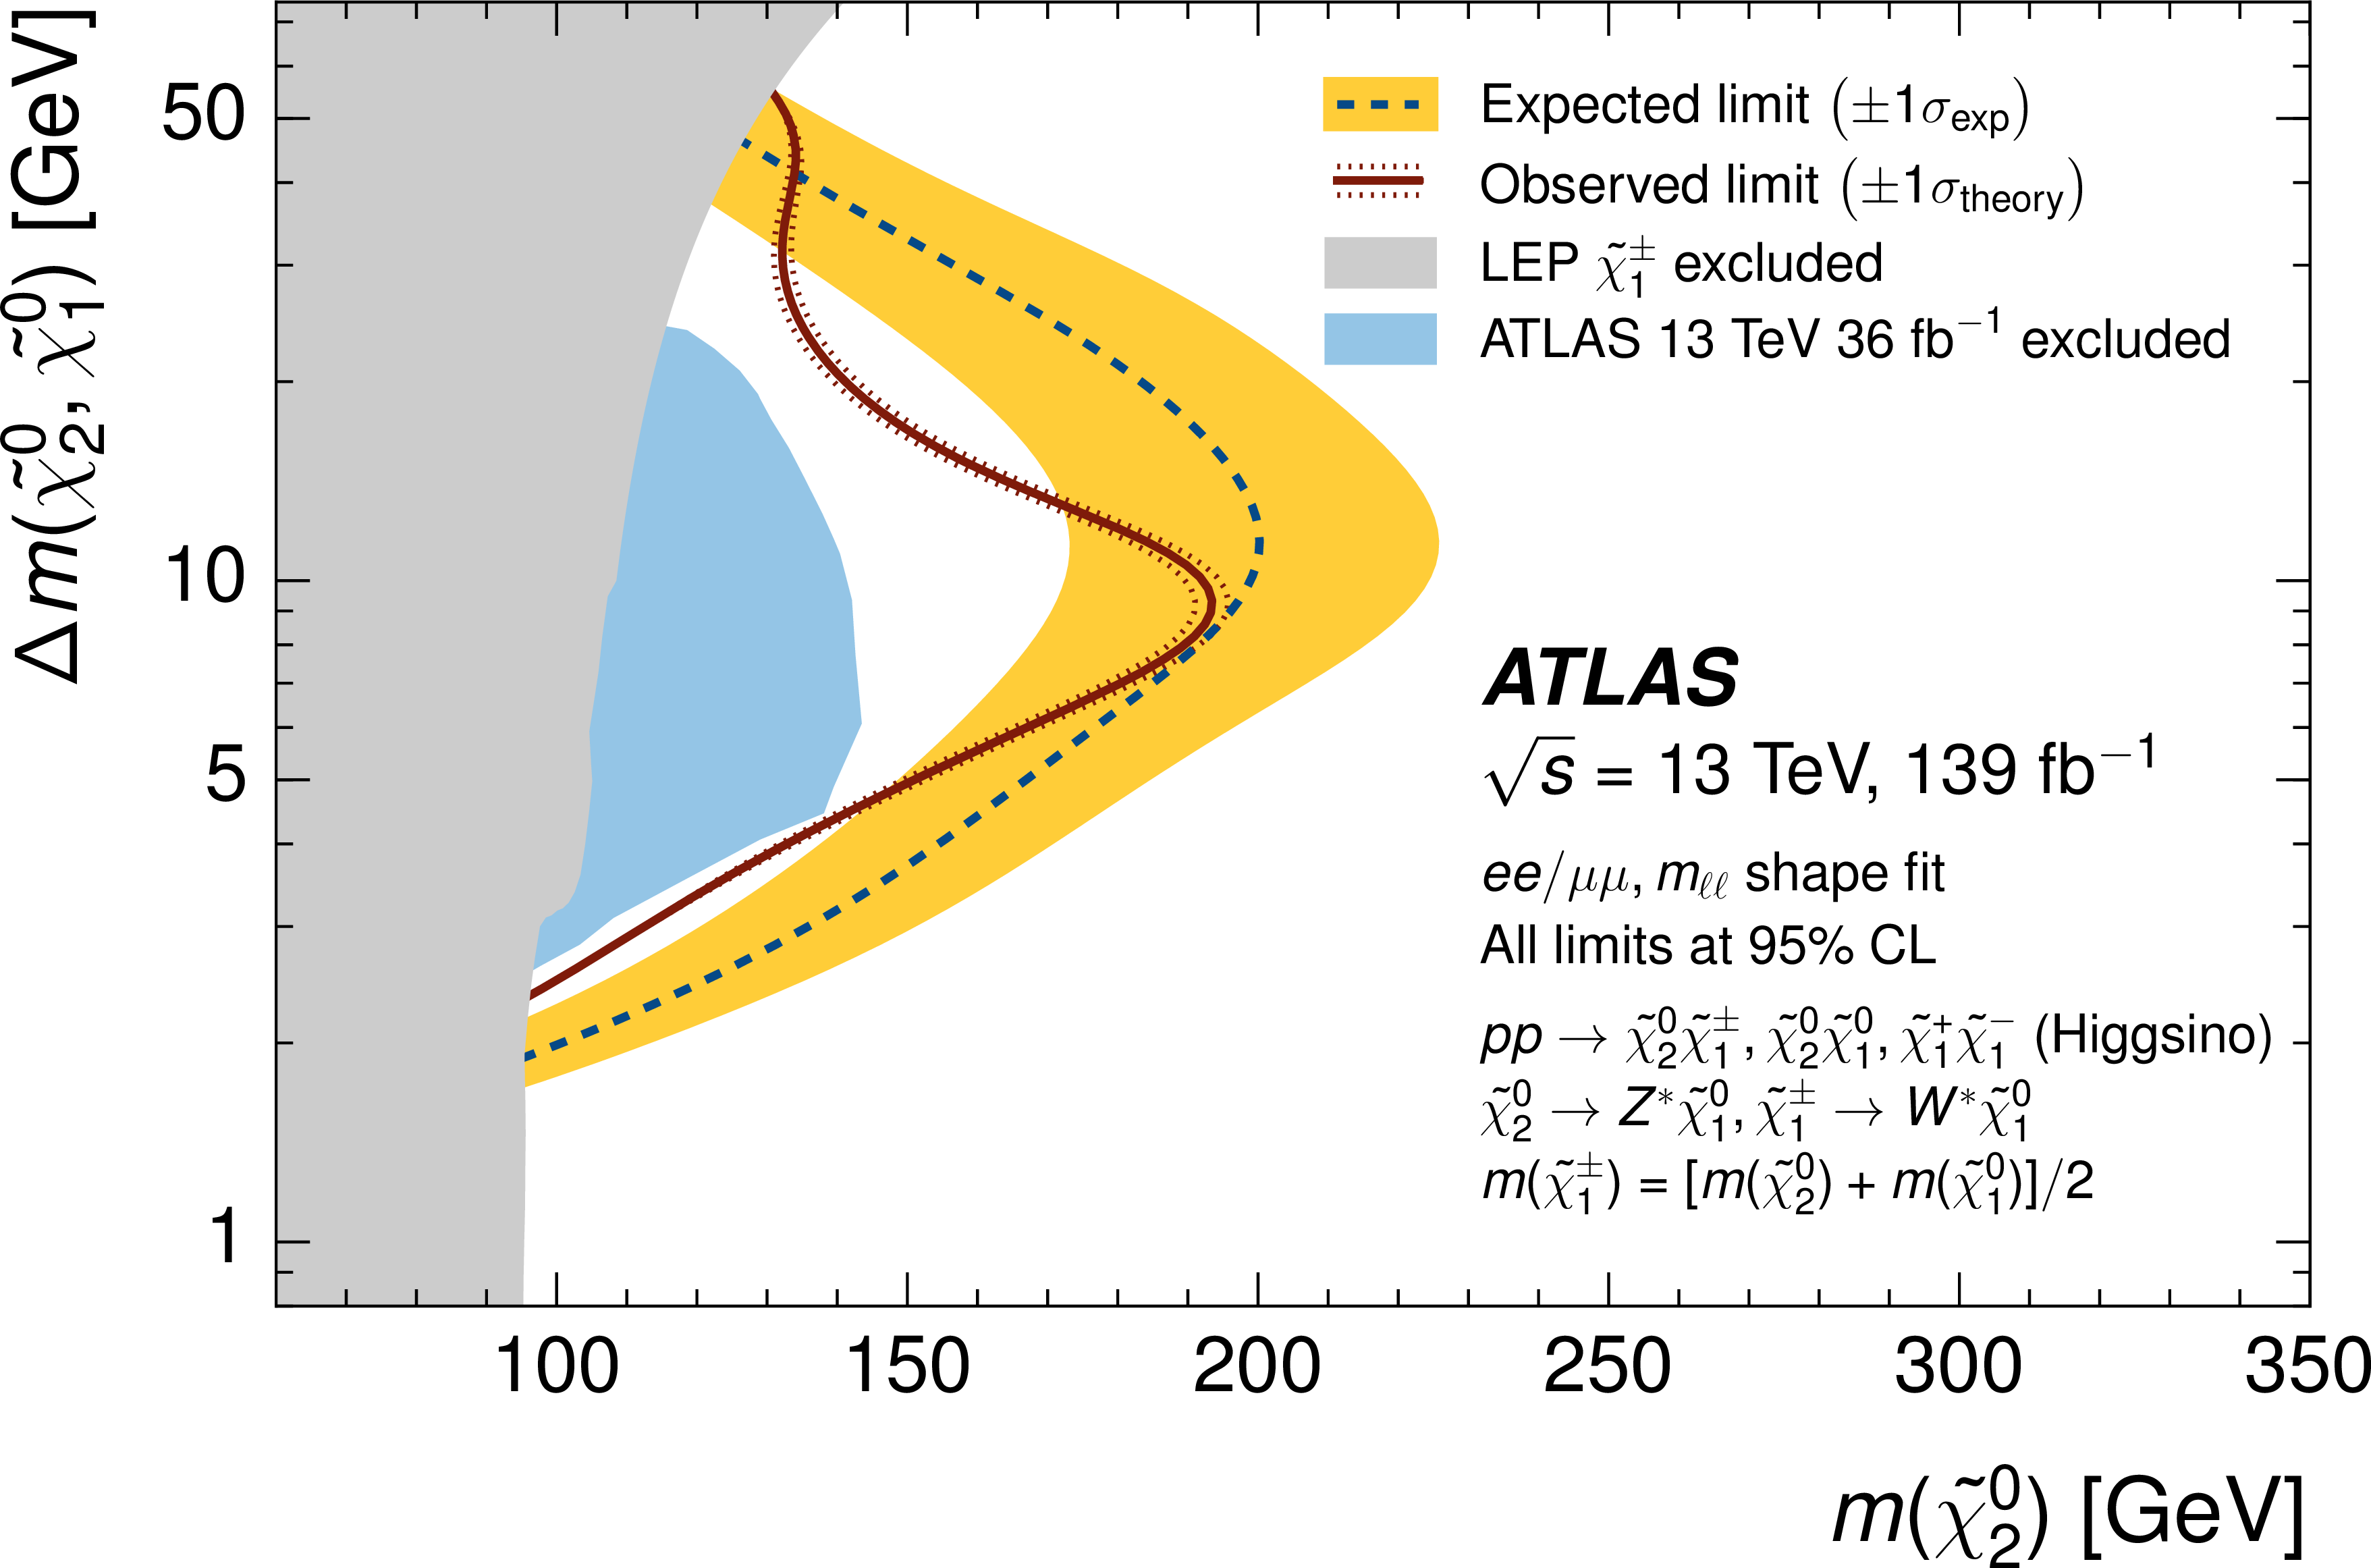
\includegraphics[width=0.48\linewidth]{plots/prev_results/ATLAS_1911_12606.png} \,
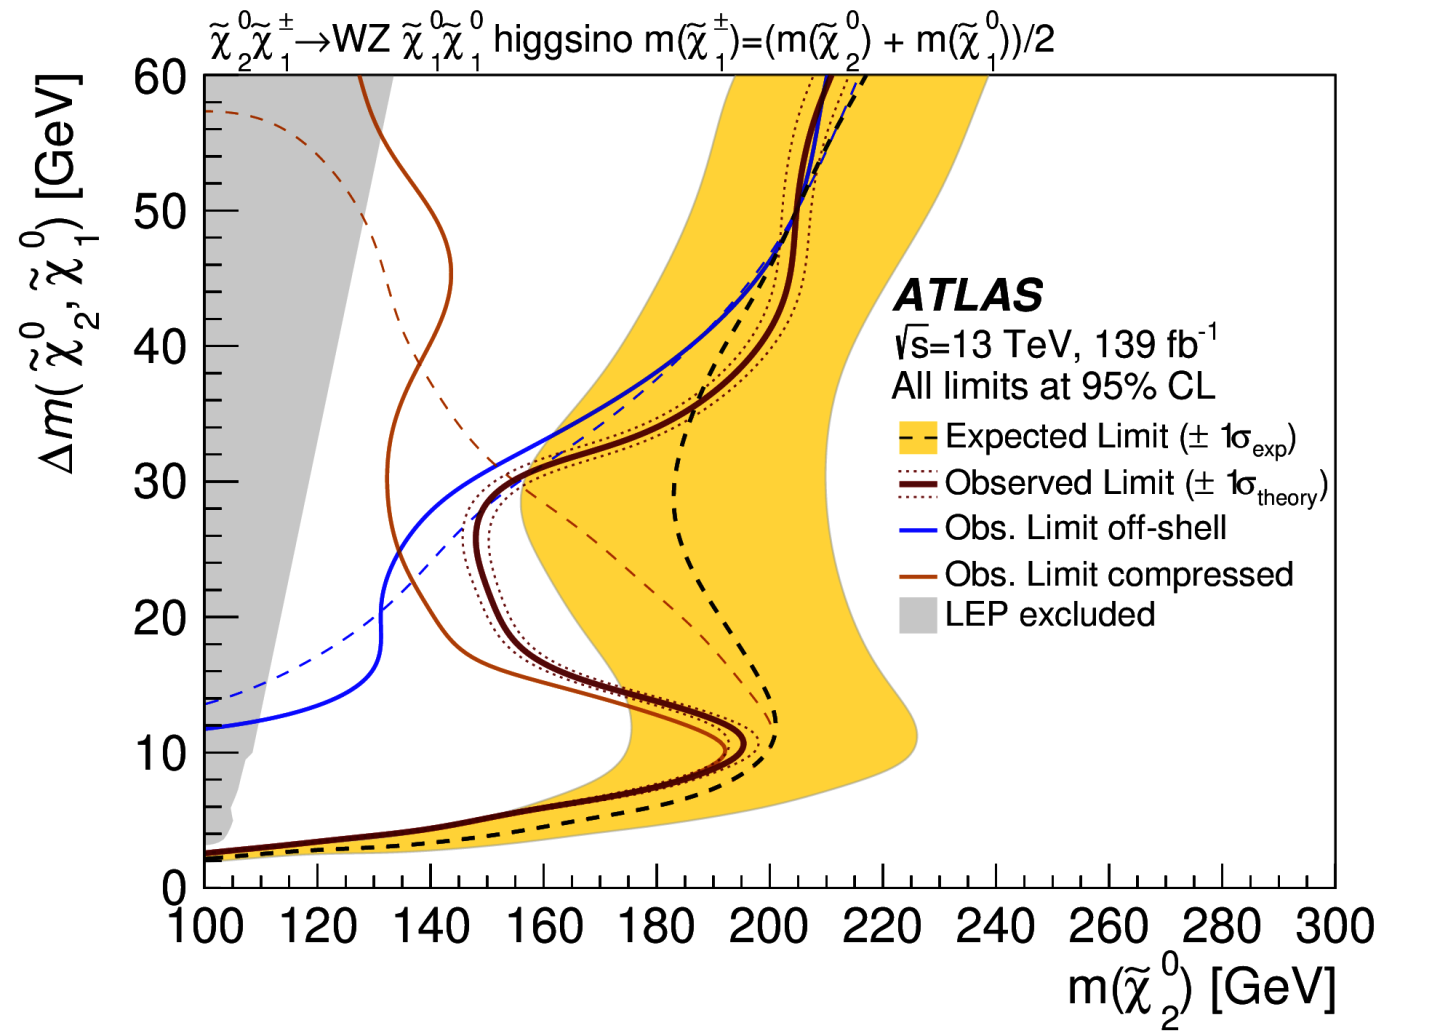
\includegraphics[width=0.48\linewidth]{plots/prev_results/ATLAS-Higgsino-combined_2106_01676.png}  \\
\caption[ATLAS higgsino production exclusion limits]{ATLAS higgsino production exclusion limits for the two lepton final state (left) and combined results for two and three lepton final state (right).}
\label{fig:atlas-limits}
\end{figure}

At CMS, search for supersymmetry in final states with two or three soft leptons and missing transverse momentum has been performed using full run 2 data~\cite{sos}. This analysis is referred to as SOS, which stands for soft opposite-sign, referring to the final state with two soft opposite-sign same-flavor leptons. Special care has been made to make the analysis presented in this thesis orthogonal the SOS analysis in order for a future statistical combination to be made possible. Therefore, there is no overlap of events between the SOS analysis, and the analysis presented in this thesis. The SOS analysis has a lower threshold on the transverse momentum of the muons of $\pt > 3.5\GeV$. It also requires the angular separation between the lepton to satisfy $\DR>0.3$. Section~\ref{sec:signal-signature} explores in detail how the analysis presented in this thesis reverts the SOS selection to make it orthogonal. In the higgsino simplified model, excluded masses reach up to $205 \GeV$ for $\dm$ of $7.5 \GeV$ and $150 \GeV$ for a highly compressed scenario with $\dm$ of $3 \GeV$. The analysis presented in this thesis attempts to extend this limit.

\begin{figure}[!htb]
\centering
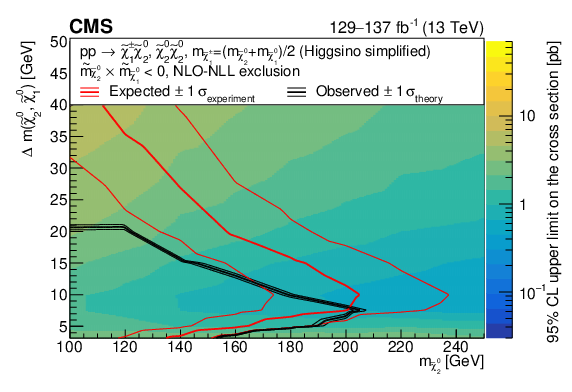
\includegraphics[width=0.80\linewidth]{plots/prev_results/cms_sos_limit.png} \\
\caption[CMS SOS higgsino production exclusion limits]{CMS higgsino production exclusion limits for the SOS analysis of final states with two or three soft leptons in a higgsino simplified model.}
\label{fig:cms-sos-limits}
\end{figure}

